% !TEX encoding = UTF-8 Unicode
\documentclass[a4paper,10pt,spanish]{article}

\usepackage[T1]{fontenc}
\usepackage[utf8]{inputenc}
\usepackage{mathtools}
\usepackage{graphicx}
\usepackage[margin=1in]{geometry}
\usepackage[spanish,activeacute]{babel}
\usepackage{hyperref}
\usepackage{fancyhdr}
\pagestyle{fancy}

\usepackage{color}
\usepackage{listings}
\lstset{ %
language=Octave,                % choose the language of the code
basicstyle=\footnotesize,       % the size of the fonts that are used for the code
numbers=left,                   % where to put the line-numbers
numberstyle=\footnotesize,      % the size of the fonts that are used for the line-numbers
stepnumber=1,                   % the step between two line-numbers. If it is 1 each line will be numbered
numbersep=5pt,                  % how far the line-numbers are from the code
backgroundcolor=\color{white},  % choose the background color. You must add \usepackage{color}
showspaces=false,               % show spaces adding particular underscores
showstringspaces=false,         % underline spaces within strings
showtabs=false,                 % show tabs within strings adding particular underscores
frame=single,           % adds a frame around the code
tabsize=2,          % sets default tabsize to 2 spaces
captionpos=b,           % sets the caption-position to bottom
breaklines=true,        % sets automatic line breaking
breakatwhitespace=false,    % sets if automatic breaks should only happen at whitespace
escapeinside={\%*}{*)}          % if you want to add a comment within your code
}
\renewcommand{\lstlistingname}{Código}
\usepackage{float}
\restylefloat{table}
\makeatletter
\def\verbatim{\small\@verbatim \frenchspacing\@vobeyspaces \@xverbatim}
\makeatother

\title{Random Sparse Matrix}

\lhead{Métodos Numéricos Avanzados}
\rhead{Random Sparse Matrix}

\begin{document}

\begin{center}
\textbf{\Huge{Random Sparse Matrix}}
\end{center}

\vspace{10mm}

\begin{center}
\textbf{INTEGRANTES: Badi Leonel, Nicolas Buchalter, Franco Depascualli, Agustin Scigliano, Marco Fallone}

\textbf{ITBA Segundo Cuatrimestre 2015}
\end{center}

\begin{center}
\text{PALABRAS CLAVE: matriz rala, random sparse matrix, mvmran, matran, autovalores, descomposición qr}
\end{center}

\vspace{10mm}

\begin{center}
\begin{large}
Resumen
\end{large}
\end{center}

Las matrices de valores dispersos(RSM) son un tipo de matriz que poseen la particularidad de tener gran cantidad de valores iguales a ceros. Conceptualmente se pueden pensar como matrices que representan sistemas donde sus elementos tienen baja cantidad de conexiones entre si, por ejemplo una red de computadoras. En este informe nos enfocaremos a analizar solamente las matrices de valores dispersos aleatorios, construidas de tal manera que tengan la misma cantidad de elementos diferentes a cero en cada columna.

\section{Introducción}
En el siguiente informe detallamos una implementación en Octave para el cálculo de autovalores en matrices RSM. Primero describiremos la implementación realizada, las decisiones que se tomaron, las dificultades que se encontraron y posibles mejoras que se pueden realizar en un futuro.

\section{Metodología}
Se decidió implementar todos los métodos en Octave ya que posee varias herramientas útiles ya implementadas para realizar operaciones con matrices (por ejemplo el producto).
Si bien para almacenar estas matrices se pueden utilizar estructuras como listas de listas o representaciones como Yale(utilización de 3 vectores), se optó por representarlas utilizando las matrices de Octave para aprovechar las ventajas antes mencionadas. También, se pensó en almacenarlas utilizando una estructura y a la hora de operar realizar una conversión a matrices de Octave. Se desestimó esta idea por el costo de procesamiento que conlleva realizar conversiones constantemente.
Para obtener los autovalores se decidió utilizar el método iterativo de QR visto en clase, con la salvedad de que en este trabajo se contemplan los casos donde los autovalores son complejos. Para determinar en que momento hace falta calcular estos valores complejos se decidió utilizar doble shifteos.

Para la descomposición QR se implemento el método de GS visto en la clase, el método modificado de GS y el método de las rotaciones de Givens.

\subsection{Implementación}
\subsubsection{Generación RSM}

Para la generación de las matrices RSM primero se generan dos matrices, una de números aleatorios y de dimensión N x NZR, la otra de ceros y de dimensiones N - NZR x N.
Luego estas matrices se concatenan una debajo de la otra para formar una matriz de dimensiones N x N. Por ultimo se itera sobre todas las columnas y se permuta de manera aleatoria las filas utilizando la función randperm de Octave.
Se puede demostrar que el orden de complejidad de esta función es \[N  O ( randperm ) \].
\begin{lstlisting}[caption = Implementación del generador de matrices RSM]
	function ret = generateRSM(N,NZR)
		A = rand(NZR,N);
		B = zeros(N-NZR,N);
		A = [A ; B];

		% Shuffle the matrix
		for i = 1:N
			ret(:,i) = A(randperm(N), i);
		end
	end
\end{lstlisting}

\subsubsection{Método QR - GS}
Como se puede ver a continuación, se implemento el método de GS propuesto por la cátedra sin realizare ninguna modificación. Este método tiene la desventaja que como genera vectores de norma pequeña, puede llevar a errores grandes en los primeros pasos que luego son arrastrados y amplifican los siguientes.

\begin{lstlisting}[caption = Implementación de la descomposición QR con GS]
	function [Q,R] = custom_qr(A)
		n = length(A);
		Q(:,1) = A(:, 1) / norm(A(:, 1));

		for i = 2 : n
			u = A(:, i);
			for j = i-1  : -1 : 1
				u = u - A(:, i)' * Q(:, j) * Q(:, j);
			end
			Q(:, i) = u / norm(u);
		end
		Q = -1*Q;
		R = Q'*A;
	end
\end{lstlisting}
\subsubsection{Método QR - GS modificado}

A continuación se muestra el método modificado de GS.

\begin{lstlisting}[caption = Implementación de la descomposición QR con GS]
	function [Q,R] = modGS_qr(A)
		R = 0;
		m = size(A)(1);
		n = size(A)(2);
		for k = 1 : n
			R(k,k) = norm(A(1:m,k));
			Q(1:m,k) = A(1:m,k) / R(k,k);
			for j=k+1 : n
				R(k,j) = Q(1:m,k)' * A(1:m,j);
				A(1:m,j) = A(1:m,j) - Q(1:m,k) * R(k,j);
			end
		end
	end
\end{lstlisting}
\subsubsection{Método QR - Rotaciones de Givens}

Dada una matriz cualquiera, se puede obtener una rotaciones de Givens tal que: \[  A=G B  \] siendo B igual a A pero con un elemento en 0. Este proceso se puede aplicar N veces para obtener una matriz triangular superior.
De esta manera podemos definir a Q como la aplicación de todas las transformadas de rotación \[ Q = G_n ... G_1  Id  \] \[ R = G_n ... G_1  A  \]

El método fue implementado siguiendo la propuesta de la cátedra, pero haciéndole una modificación para que se calcule correctamente Q.

\begin{lstlisting}[caption = Implementación de la descomposición QR con GS]
	function [Q,R] = givens_qr(A)
		R = A;
		m = size(A)(1);
		n = size(A)(2);
		Q = eye(m,n);
		for k = 1 : n
			for l = k +1 : m
				if (R(l,k) == 0)
					c = 1;
					s = 0;
				elseif abs(R(l,k)) < abs(R(k,k))
					t = R(l,k) / R(k,k);
					c = 1 / sqrt(1+t^2);
					s = c * t;
				else
					z = R(k,k) / R(l,k);
					s = 1/ sqrt(1 + z^2);
					c = s*z;
				end
				G = [c,s; -s,c];
				R([k,l] , k:n) = G * R([k,l], k : n);
				Q([k,l] , 1:n) = G * Q([k,l], 1:n);
			end
		end
		Q = Q';
	end
\end{lstlisting}




\subsubsection{Método eig}

Luego de implementar la descomposición QR, se prosiguió a implementar la función \texttt{eig}. Primero se utiliza el algoritmo generateRSM antes implementado para generar una matriz de valores dispersos, a la cual llamamos A. Luego, iterativamente se realiza la descomposición QR de A, utilizando alguno de los métodos antes propuestos y luego A = RQ. Se evalúan los elementos (matrices de 2x2) de la diagonal para calcular los autovalores. El elemento inferior izquierdo de cada matriz de la diagonal es comparado con la suma de dos elementos de la diagonal multiplicado por una tolerancia o error. En particular si el elemento : \[A_i_{j-1} < error ( | A_i_j | + | A_{i-1}_{j-1} |) \] hay que obtener un auto-valor real. Si esto no sucede pero : \[A_i_{j-1} < error ( | A_{i-2}_{j-2} | + | A_{i-1}_{j-1} |) \] hay que obtener un valor complejo obteniendo los autovalores de una matriz de 2x2. Si ninguna de estas cosas suceden hay que seguir iterando. Cada vez que obtenemos un autovalor reducimos la matriz ya que los valores convergen de abajo para arriba.

\begin{lstlisting}[caption = Obtención de Autovalores]

function [values, timeElapsed] = qr_eig(firstA,error,qr_method)
  more off;
  A = firstA;
  n = length(A);
  tic;
  actual_value = 0;
  do
    prevA = A;
    [Q, R] = qr_method(prevA);
    A = R * Q;
    if (abs(A(n-actual_value,n-actual_value-1)) < error*(abs(A(n-actual_value-1,n-actual_value-1))+abs(A(n-actual_value,n-actual_value)))) %Shif
      values(n-actual_value,1) = A(n-actual_value,n-actual_value);
      A = A(1:n-actual_value-1, 1:n-actual_value-1);
      actual_value = actual_value+1;

    elseif (abs(A(n-actual_value-1,n-actual_value-2)) < error*(abs(A(n-actual_value-1,n-actual_value-1))+abs(A(n-actual_value-2,n-actual_value-2)))) %Double-Shif
      a = A(n-actual_value-1,n-actual_value-1);
      b = A(n-actual_value-1,n-actual_value);
      c = A(n-actual_value,n-actual_value-1);
      d = A(n-actual_value,n-actual_value);
      [x1, x2] = cuadratic_eq(1, -a-d, a*d - c*b);
      values(n-actual_value-1,1) = x1;
      values(n-actual_value,1) = x2;

      A = A(1:n-actual_value-2, 1:n-actual_value-2);
      actual_value = actual_value + 2;
    end
  until(actual_value >= n-2);
  if(actual_value == n-2)
      a = A(n-actual_value-1,n-actual_value-1);
      b = A(n-actual_value-1,n-actual_value);
      c = A(n-actual_value,n-actual_value-1);
      d = A(n-actual_value,n-actual_value);
      [x1, x2] = cuadratic_eq(1, -a-d, a*d - c*b);
      values(n-actual_value-1,1) = x1;
      values(n-actual_value,1) = x2;
      A = A(1:n-actual_value-2, 1:n-actual_value-2);
  elseif(actual_value == n-1)
    values(1) = A(1,1);
  end
  timeElapsed = toc();
end

\end{lstlisting}

\pagebreak

\section{Resultados}

\begin{figure}[!htb]
    \centering
    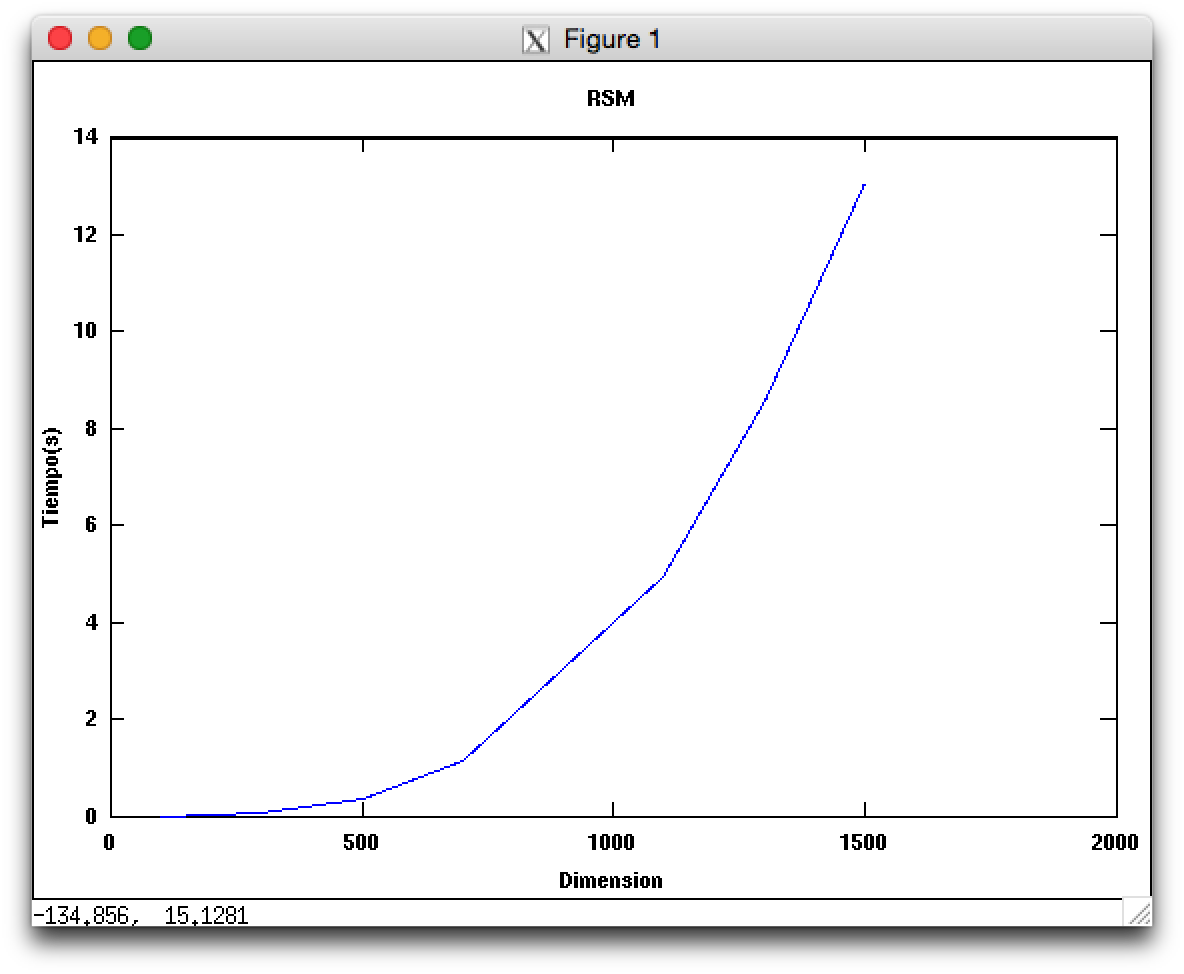
\includegraphics[width=120mm]{GenerateRSM.png} 
    \caption{Eficiencia del método GenerateRSM, con 20\% de los valores de la columna distintos a 0}
\end{figure}

\begin{figure}[!htb]
    \centering
    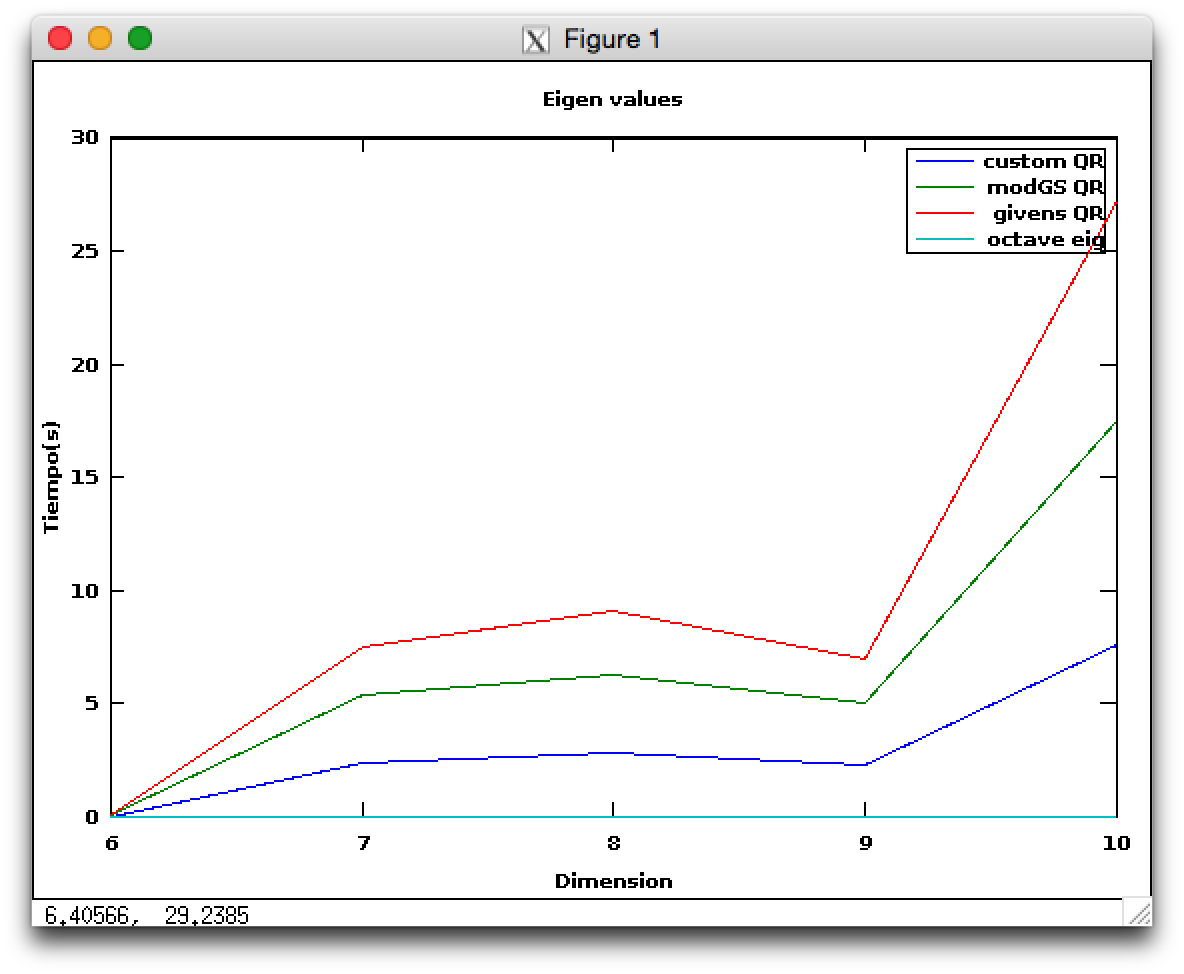
\includegraphics[width=120mm]{eig_comp.png}  
    \caption{Eficiencia en el calculo de autovalores}
\end{figure}

\begin{center}
\begin{table}[!htbp]
\centering
\begin{tabular}{cc}
\hline
\textbf{Dimensión (nxn)} & \textbf{Tiempo (sec)} \\ \hline
50											& 29								\\
100											& 656								\\
200											& 10800+							\\
\end{tabular}
\caption[Eficiencia en el calculo de autovalores] {Tiempo hasta obtener los autovalores.}
\end{table}
\end{center}

Se puede ver en la figura 1 que el método para generar la matriz RSM no aumenta de manera lineal con respecto a las dimensiones de la matriz. Este comportamiento cuadrático era de esperarse ya que utilizamos la función de Octave randperm dentro de un ciclo.


La figura 2 es un modelo representativo del tiempo requerido para calcular los autovalores. Se encuentra disponible el script testEigScript en el cual se pueden modificar los parámetros para realizar el análisis de los métodos para calcular autovalores. En todos los casos el método QR con GS resultó el mas eficiente. Cabe resaltar que eig() de octave resultó considerablemente mas eficiente que los métodos implementados, generalmente alrededor de cinco ordenes de magnitud de diferencia. El error utilizado fue en todos los casos 0.00001.

En la tabla 1 se puede observar el tiempo transcurrido hasta obtener los autovalores utilizando el método de descomposición QR de GS. El NZR para todos los casos es de un 20\% de N.

\pagebreak

\section{Conclusiones}
Como conclusión, logramos obtener correctamente los autovalores de una matriz RSM de hasta una dimensión de un N=100. También podemos concluir que la eficiencia de la descomposición QR para calcular autovalores utilizando este método es determinante, ya que es un proceso que se va a estar realizando constantemente. Si deberíamos seguir optimizando este proceso , habría que rever las implementaciones de la descomposición QR utilizada.

Intentamos obtener los autovalores de una matriz de 200x200 pero luego de dos horas corriendo solo pudo sacar los primeros 43 autovalores. Hay que considerar que todas las pruebas se realizaron con un error de 0.00001.

Algo que nos sorprendió es que la descomposición por rotaciones de Givens dio mayores tiempo que la descomposición de GS. Esto nos hace pensar que hay una manera mucho mas efectiva de implementarla (Como Fast-Givens).

Otra cosa que llama la atención es el tiempo despreciable que tiene Octave en comparación con nuestros métodos. Esto nos hace pensar que hay muchas optimizaciones que mejoren considerablemente la complejidad del método. También esta la posibilidad de que se utilice un enfoque diferente.

\pagebreak

\section{Bibliografía}
\begin{itemize}

\item Apuntes de las clases teórica y práctica de la materia Métodos Numéricos Avanzados (Segundo Cuatrimestre, 2015).

\item Documento sobre descomposición QR proporcionado por la cátedra de Métodos Numéricos Avanzados (Segundo Cuatrimestre, 2015).

\item \url{http://www.win.tue.nl/casa/meetings/seminar/previous/_abstract051109_files/presentation_full.pdf}

\item \url{http://people.inf.ethz.ch/arbenz/ewp/Lnotes/chapter3.pdf}

\end{itemize}

\pagebreak

\end{document}